\begin{figure}[ht!]
\centering
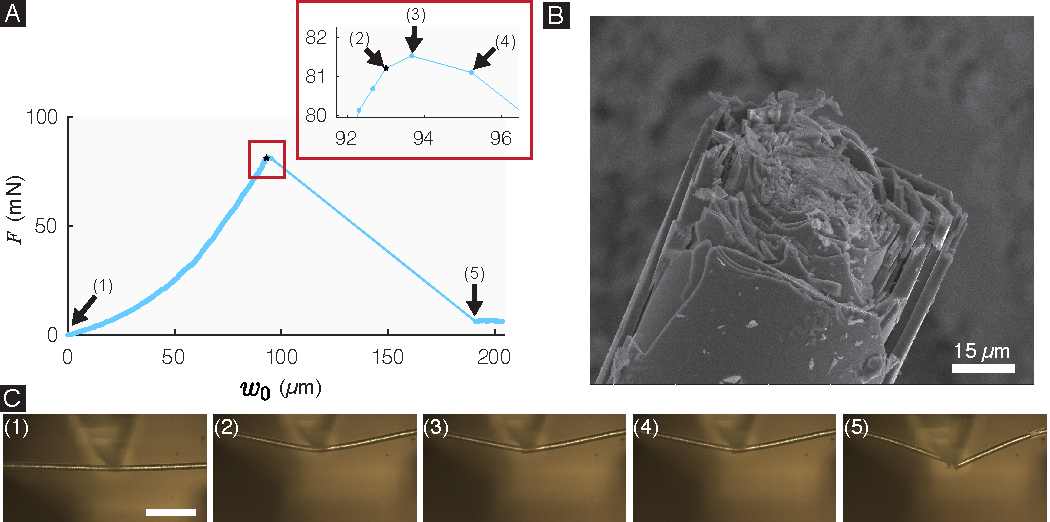
\includegraphics[width=\textwidth]{Figures/Figure4_V3.pdf}
\caption{Force-displacement response from fixed-fixed three-point bending tests. (\textsf{A}) The force $F$ as a function of mid span specimen displacement $w_0$ for a representative spicule tested in the fixed-fixed setup. The inset shows a zoomed view of the plot region within the red square. (\textsf{B}) A micrograph of the broken end of the spicule whose $F$-$w_0 $ data is shown in (\textsf{A}). (\textsf{C}) Micrographs taken during the three-point bending test of the spicule. The numbers correspond to the numbered ($w_0$, $F$) points shown in (\textsf{A}). The scale bar in (1) measures 250 $\mu$m and micrographs (2)--(5) have the same scale as (1). In (1), the spicule is in the reference configuration. Images (2)--(4) show the onset of failure in the spicule and image (5) shows the complete failure of the spicule. The failure process ((2)--(4)) occurs over only 3 stage displacement increments and does not display the sawtooth pattern observed in the tests performed using the simply-supported setup (see Figures~\ref{fig:SSconfig} (\textsf{F}) and~\ref{fig:slip} (\textsf{D})).}
\label{fig:TPBF}
\end{figure}
